
\chapter{Aplicaciones lineales $\divideontimes$}	


\section{Homomorfismos}	


El objetivo de este capítulo es el estudio de las aplicaciones lineales u homomorfismos entre espacios vectoriales. Este tipo de aplicaciones respeta la estructura de espacio vectorial transformando subespacios vectoriales en subespacios vectoriales. 


\begin{defi}
Sean $V \text{ y } V'$	dos subespacios vectoriales, una aplicación $f\,: \; V \; \to \; V'$ se dice que es una `aplicación lineal' u \emph{homomorfismo} si:

$\forall \vec u, \vec v \in V ; \; \forall \alpha, \beta \in \mathbb R \; : \quad $ \colorbox{LightYellow}{$\boxed{\; f\;(\;\alpha \vec u + \beta \vec v \; )= \alpha\; f(\vec u) + \beta \; f (\vec v)\; }$}
\end{defi}

\begin{ejem}.
	
\noindent --- $I:V\to V\; / \; I(\vec v)=\vec v,\; \forall \vec v \in V$ es, trivialmente, una aplicación lineal.

\noindent --- $f:\mathbb R^2 \to \mathbb R^3\; / \; f(x,y)=(x,x+y,x-2y)$ es una aplicación lineal:

\noindent $ f(\; \alpha(x_1,y_1)+\beta(x_2,y_2)\; )= f(\; \alpha x_1+\beta x_2\; , \; \alpha y_1+\beta y_2\; ) =$

\noindent $= (\; \alpha x_1 + \beta x_2 \; , \; \alpha x_1+\alpha y_1 + \beta x_2 + \beta y_2 \; , \; \alpha x_1+\beta x_2-2\alpha y_1 - 2 \beta y_2\; )=   $

\noindent $=\alpha\cdot (\; x_1, x_1+y_1, x_1-2y_1 \;)  +\beta \cdot (\; x_2, x_2+y_2, x_2-2y_2 \;) = $

\noindent $=\alpha \; f(x_1,y_1)+\beta \; f(x_2,y_2) $

\noindent --- $g:\mathbb R^2 \to \mathbb R^3 \; :\quad g(x,y)=(x^2, x+y,x-2y)$, no es una aplicación lineal pues (contraejemplo):

\noindent $g(\;(-1)\cdot (1,1) \;)= (1,-2,1); \quad (-1)\cdot g(1,1)=(-1)(1,2,-1)=(-1,-2,1) \Rightarrow g(\;(-1)\cdot (1,1) \;) \neq (-1)\cdot g(1,1)$

\noindent --- $h: \mathbb R^2 \to \mathcal M_{2 \times 2}(\mathbb R)\; : \quad h(x,y)=\left( \begin{matrix} x&0\\1&y \end{matrix} \right)$, no es una aplicación lineal.

\noindent $h(\; (x_1,y_1)+(x_2,y_2)\; )=\left( \begin{matrix} x _1+x_2&0\\1&y_1+y_2 \end{matrix} \right) \neq \left( \begin{matrix} x _1&0\\1&y_1 \end{matrix} \right) + \left( \begin{matrix} x_2&0\\1&y_2 \end{matrix} \right)=h(x_1,y_1)+h(x_2,y_2)$

\end{ejem}

Por su importante significado geométrico, destacamos \underline{algunas aplicaciones} \underline{lineales importantes}:

\begin{itemize}

\item \textbf{Aplicación identidad}: asigna a cada vector el mismo vector. 

$I:V\to V\;:\; I(\vec v)=\vec v$

\item \textbf{Aplicación nula}: siempre asocia el vector nulo del subespacio imagen.

$N:V \to V'\; :\; N(\vec v)=\vec 0_{V'}$

\item \textbf{Giros ángulo $\theta$}: Provoca un giro de $\theta$ grados sobre el vector.

$G_{\theta}: \mathbb R^2 \to \mathbb R^2 \; : \; G_{\theta} (x,y)= (\cos \theta \;x - \sin \theta \;y \;,\; \sin \theta \;x + \cos \theta \;y)$

\item \textbf{Reflexiones o simetrías}: un ejemplo de simetría en el espacio respecto del plano $XZ$ sería,

$S_{XZ}:\mathbb R^3 \to \mathbb R^3 \: :\; S_{_{XZ}}(x,y,z)=(x,-y,z)$

\item \textbf{Homotecias}: Producto de un escalar por un vector (si el escalar es, en módulo mayor que $1$ tenemos una dilatación; si es menor, una contracción). Como ejemplo pondremos la dilatación (superficial) de una lámina del $1\%$ debido al calor,

$D:\mathbb R^3 \to \mathbb R^3\; : \; D(x,y)=(1.01x, 1.01y)$

\item \textbf{Proyecciones}: Son aplicaciones que llevan todos los vectores de $\mathbb R^3$ a un plano sobre el que se proyecta. P.e., una proyección sobre el plano $YZ$ sería,

$P:\mathbb R^3 \to \mathbb R^3\; :\; P(x,y,z)=(x,0,z)$

\end{itemize}

\begin{defi}
Una aplicación lineal $\; f:V\to V'$ se dice que es:
\begin{itemize}
\item \textbf{inyectiva} si $\; f(\vec u)=f(\vec v) \longrightarrow \vec u = \vec v$, de otro modo, a originales distintos le corresponden imágenes distintas.
\item \textbf{epiyectiva, sobreyectica o suprayectica} si $\forall \vec v' \in V' \; \exists \vec v \in V\; / \; \vec v' = f(\vec v)$, es decir, si $f(V)=V'$
\item Si $f$ es inyectiva y epiyectiva se dice que es \textbf{biyectiva}	
\end{itemize}
	
\end{defi}

\begin{ejem}.

--- La aplicación del conjunto de la población española mayor de edad en $\mathbb N$ que asocia a cada ciudadano su DNI es INYECTIVA, pues no hay dos personas con el mismo DNI. Pero NO es EPIYECTIVA	porque no se usan todos los números naturales.

--- La aplicación de $\mathbb R$ en $\mathbb R^+$ que asocia a cada número real su cuadrado NO es INYECTIVA pues a los números opuestos les asocia en mismo cuadrado ($(2^2=(-2)^2=4$), pero sí es EPIYECTIVA ya que todos los números reales positivos son el cuadrado de algún número real.
\end{ejem}

\justify

Dependiendo de sus características las aplicaciones lineales (\textbf{homomor-fismos}) $f:V\to V'$ se clasifican en:

\begin{itemize}
\item MONOMORFISMO: si $f$ es inyectiva.
\item EPIMORFISMO: si $f$ es epiyectiva.
\item ISOMORFISMO: si $f$ es biyectiva.
\item ENDOMORFISMO: si $V=V'$
\item AUTOMORFISMO: si $V=V'$ y $f$ es biyectiva.
\end{itemize}

\section{Subespacios de una aplicación lineal.}

Las aplicaciones lineales transforman subespacios vectoriales en subsespacios vectoriales (conservan la estructura de subespacio vectorial):

\subsection{Subespacio \emph{Imagen} de una aplicación lineal}

\begin{prop}
$f:V\to V'$, sea $W \subseteq V$ un subespacio vectorial, entonces $f(W)=\{f(\vec u): \; \vec u\in W \}$	 es un subespacio vectorial de $V'$.
\end{prop}
\begin{proof}
\textcolor{gris}{ $\alpha, \beta \in \mathbb R; \; \vec u, \vec v \in f(W) \to \exists \vec u_1, \vec v_1 \in W \; / \; f(\vec u_1)=\vec u\; \wedge \; f(\vec v_1)=\vec v \Rightarrow \alpha\; \vec u + \beta\; \vec v = \alpha\; f(\vec u_1) + \beta\; f(\vec v_1) =f(\alpha\; \vec u_1+\beta \; \vec v_1)$, por lo que $ \alpha\; \vec u + \beta \; \vec v \in f(W)$ }	
\end{proof}

\begin{defi}
Dada $f:V\to V'$ aplicación lineal, se llama \textbf{imagen} de f, $\;Im(f)\;$, al conjunto $f(V)$ que, como se ha visto en la proposición anterior, es un subespacio vectorial de $V'$. Además, se cumple que: 

$f$ es \emph{epimorfismo} $\leftrightarrow Im(f)=V'$	 

------ La $Im(f)$ permite clasificar a los epimosfismos (aplicaciones epiyectivas o suprayectivas).
\end{defi}

\begin{ejem}
$f:\mathbb R^3 \to \mathbb R^3\;.\quad f(x,y,z)=(x+y,x-z,2x+y-z)$

\noindent $(x,y,z)\in Im(f) \text{ si } \exists (\alpha, \beta, \gamma)\in\mathbb R^3 \: : \quad (x,y,z)=f(\alpha, \beta, \gamma)=$

\noindent $=(\alpha+\beta, \alpha -\gamma, 2\alpha+\beta-\gamma)  \to \begin{cases} \alpha+\beta&=x\\ \alpha -\gamma&=y\\ 2\alpha+\beta-\gamma&=z \end{cases}$, ha de ser SC.

\noindent \textcolor{gris}{(\emph{ecuaciones paramétricas de $Im(f)$})}, calculando rangos por Gauss (p.e.):

\noindent \small{$\left( \begin{matrix} 1&1&0\\1&0&-1\\2&1&-1 \end{matrix} \right| \left. \begin{matrix} x\\y\\z \end{matrix} \right) \to  \left( \begin{matrix} 1&1&0\\0&-1&-1\\0&-1&-1 \end{matrix} \right| \left. \begin{matrix} x\\y-x\\z-2x \end{matrix} \right) \to \left( \begin{matrix} \boxed{1}&\boxed{1}&0\\\boxed{0}&\boxed{-1}&-1\\0&0&0 \end{matrix} \right| \left. \begin{matrix} x\\y-x\\z-2-y \end{matrix} \right) $}

\noindent \normalsize{al} exigir que los rangos de matrices de coeficientes y ampliada sean iguales a $2:\qquad z-x-y=0\;$, por lo que:

 $Im(f)=\{\;\ (x,y,z)\in \mathbb R^3\; : \quad z-x-y=0 \; \}$ \textcolor{gris}{(\emph{ecuación implícita de $Im(f)$})}.
\end{ejem}

Veamos un método alternativo de calcular $Im(f)$:

\begin{prop}
Sean $f:V\to V'$, aplicación lineal y $B=\{ \vec u_1, \cdots , \vec u_n \}$ una base de $V$, entonces $f(B)$ es un sistema generador de $Im(f)$.
\end{prop}

\begin{proof}
\textcolor{gris}{ Sea $\vec v\in Im(f) \to \exists \vec u \in V\ \therefore \; \vec v=f(\vec u)$. Como $B$ es base de $V$, existen $\alpha_1, \cdots , \alpha_n \in \mathbb R \; / \; \vec v = f(\vec u)= f(\alpha_1\; \vec u_1 + \cdots + \alpha_n\; \vec u_n)=\alpha_1 f(\vec u_1)	+ \cdots + \alpha_n f(\vec u_n)$, por lo que $f(B)$ genera el subespacio imagen $Im(f)$.}
\end{proof}

\begin{ejem} Calculemos, de otro modo $Im(f)$ del ejemplo anterior:

\noindent $f:\mathbb R^3 \to \mathbb R^3\;.\quad f(x,y,z)=(x+y,x-z,2x+y-z)$

\noindent$C=\{\; (1,0,0),(0,1,0),(0,0,1) \;\}$ es la base canónica de $\mathbb R^3$, calculamos $f(C)=\{\; (1,1,2),(1,0,1),(0,-1,.1) \;\}$, 

\noindent entonces $Im(f)=\mathcal L(\; \{\; (1,1,2),(1,0,1),(0,-1,-1) \;\} \; )$, es decir,

\noindent $(x,y,z)\in Im(f) \leftrightarrow \exists \; \alpha, \beta, \gamma \in \mathbb R\; \therefore \;$ 

\noindent $ (x,y,z)= \alpha (1,1,2)+ \beta (1,0,1) + \gamma (0,-1,-1)= (\alpha+\beta , \alpha-\gamma, 2\alpha+\beta-\gamma)$, que son las ecuaciones paramétricas de $Im(f)$ obtenidas en el ejemplo anterior. Si eliminamos los parámetros, como allí, obtendríamos:

\noindent  $z-x-y=0$ como ecuación implícita de $Im(f)$.
	
\end{ejem}



\subsection{Subespacio \emph{Núcleo} de una aplicación lineal}

\begin{defi}
Sea $f:V \to V'$ una aplicación lineal, se llama \textbf{núcleo}	 de f, $ker(f)$ \textcolor{gris}{ (de `kernel', de la raíz germánica Kern, núcleo) }, a los vectores de $V$ cuya imagen por $f$ es el $\vec 0 \;\in V':$

$Ker(f)=\{\; \vec u \in V \; : \; f(\vec u)=\vec 0 \textcolor{gris}{\; \in V'} \;\}$

\end{defi}

\begin{prop}
El núcleo de una aplicación lineal $f:V \to V'$, $\;\ker(f)\;$,	es un subespacio vectorial de $V$
\end{prop}
\begin{proof}
\textcolor{gris}{$\alpha, \beta \in \mathbb R; \; \vec u, \vec v \in ker(f): \; f(\vec u)=f(\vec v)=0 \to $}

\noindent \textcolor{gris}{$f(\alpha \vec u + \beta \vec v)=\alpha f(\vec u)+ \beta f(\vec v)  = \alpha \; \vec 0 + \beta \vec 0=\vec 0 \Rightarrow  (\alpha \vec u + \beta \vec v)\; \in ker(f)$}
\end{proof}

------ El núcleo permite caracterizar a los monomorfismos (aplicaciones inyectivas).

\begin{prop}
	Sea $f:V\to V'$ aplic. lineal. 
	
	Entonces, $f$ es inyectiva $\leftrightarrow Kerf(f)=\vec 0$
\end{prop}
\begin{proof}
\textcolor{gris}{ f inyectiva $\to  \vec u \in ker(f):\; f(\vec u)=\vec 0=f(\vec 0)$ y por inyectividad, $\vec u = \vec 0 \to Ker(f)=\{ \vec 0 \} $. Recíprocamente, si $Ker(f)=\{\vec 0 \} \text { y } f(\vec u)=f(\vec v),$ por linealidad, $\vec 0= f(\vec u)-f(\vec v)=f(\vec u - \vec v) \to \vec u-\vec v \in Kerf(f)=\{\vec 0\} \to \vec u=\vec v$  }	
\end{proof}

\begin{teor}
Sea $f:V \to V'$ una aplicación lineal de un espacio vectorial $V$ de dimensión finita en un espacio vectorial $V'$, se verifica la igualdad:

\begin{equation*}
	\colorbox{LightYellow}{\boxed{ \; dim(V)\; =\; dim \; Kem(f)\; +\; dim \; Im(f)\; }}
\end{equation*}	
\end{teor}

\begin{ejem}
$f:\mathbb R^3 \to 	\mathbb R^3\; : \quad f(x,y,z)=(x-y,x-z,-y-z)$. Calcula su núcleo y si imagen.

\noindent $(x,y,z) \in Ker (f) \leftrightarrow (0,0,0)= f(x,y,z)=(x-y,x-z,-y-z) \to \begin{cases} x-y=0 \\ x-z=0 \\ -y-z=0 \end{cases} \to SCD \text{ homog.} \to x=y=z=0 \Rightarrow $

\noindent $Ker(f)=\{(0,0,0\} \text{ y } dim\; ker(f)=0 \to dim\; Im(f)=3 \Rightarrow Im(f)=\mathbb R^3$
\end{ejem}

\section{Matriz asociada a una aplicación lineal}

Sea $f:V\to V'$ una aplicación lineal y sen $B=\{ \vec u_1, \cdots, \vec u_m \} $ y $B'=\{ \vec v_1, \cdots, \vec v_n \} $ dos bases de $V$ y $V'$ respectivamente. Dado un vector cualquiera $\vec u\in V$, existen $m$ escalares $\alpha_1, \cdots, \alpha_m \in \mathbb R$ de forma que: $\vec u = \alpha_1\; \vec u_1 + \cdots + \alpha_m\; \vec u_m$ \textcolor{gris}{(Estos $\alpha_i; \; 1\le i \le m$ son las componentes de $\vec u$ en la base $B$)} y por linealidad de $f$ tenemos que: 

$f(\vec u)=\alpha_1\cdot f(\vec u_1) + \cdots + \alpha_m\cdot f(\vec u_m)$

De donde se deduce que conociendo las imágenes por una aplicación lineal de ls vectores de una base del espacio inicial, es posible calcular la imagen que se obtiene por la aplicación lineal de cualquier vector. Por otra parte, $f(\vec u_1), \cdots, f(\vec u_m)$ estan en $V'$, por lo que pueden escribirse como combinación lineal de los vectores de una de sus bases, $B'$. Sean $\lambda_{1j}, \cdots, \lambda_{nj}\; \in \mathbb R$ las coordenadas de $f(\vec u_j)$ en $B'$, es decir,

$f(\vec u_j)=\lambda_{1j}\cdot f(\vec v_1) + \cdots + \lambda_{nj}\cdot f(\vec v_n)\; , \quad 1\le j \le m$, se tiene:

$\displaystyle f(\vec u)= \sum_{j=1}^m \alpha_{j}\cdot f(\vec u_j)=\sum_{j=1}^m \alpha_j \left( \sum_{i=1}^n \lambda_{ij}\cdot \vec v_i \right)=\sum_{i=1}^n \left( \sum_{j=1}^m \lambda_{ij} \; \alpha_j \right) \; \vec v_i$
 
 Si $\beta_1, \cdots, \beta_n\; \in \mathbb R$ son las componentes del vector $f(\vec u)$ en la base $B'$, como se trata de una base y un vector se escribe en ella de farma única:
 
 $\displaystyle \beta_i=\sum_{j=1}^m \lambda_{ij} \; \alpha_j \; , \quad 1\le i \le n\; $, matricialmente:
 
 $M_{BB'}(f)= \left(  \begin{matrix}  \lambda_{11} &  \lambda_{12}& \cdots &  \lambda_{1m} \\  \lambda_{21}& \lambda_{22}&\cdots & \lambda_{2m}\\ \vdots & \vdots & \ddots & \vdots \\  \lambda_{n1}& \lambda_{n2}&\cdots&  \lambda_{nm} \end{matrix}  \right)\; \in\; \mathcal M_{n \times m} (\mathbb R)$ , 
 
 cuyas columnas son las componentes en $B'$ de las imágenes por $f$ de los vectores $f(\vec u_i)$, con lo que:
 
 $\left( \begin{matrix} \beta_1 \\ \beta_2 \\ \vdots \\ \beta_n \end{matrix} \right) =   \left(  \begin{matrix}  \lambda_{11} &  \lambda_{12}& \cdots &  \lambda_{1m} \\  \lambda_{21}& \lambda_{22}&\cdots & \lambda_{2m}\\ \vdots & \vdots & \ddots & \vdots \\  \lambda_{n1}& \lambda_{n2}&\cdots&  \lambda_{nm} \end{matrix}  \right) \cdot \left( \begin{matrix} \alpha_1 \\ \alpha_2 \\ \vdots \\ \alpha_m \end{matrix} \right)$
 
 La matriz $M_{BB'}f$ es la \textbf{matriz de la aplicación $\boldsymbol{f}$ en las bases $\boldsymbol{B}$ y $\boldsymbol{B'}$} y permite obtener en la base $B'$ la imagen por $f$ de cualquier vector a partir de sus componentes es la base $B$, como se indica en la relación anterior.
 
 \begin{ejem}
 	Sean $f:\mathbb R^2 \to \mathbb R^3\; : \quad f(x,y)=(x,x+y.x-2y)$, una aplicación lineal; $\; C_2,\; C_3$ las bases canónicas de $\mathbb R^2 \text{ y } \mathbb R^3$.
 	
 \noindent $f(1,0)=(1,1,1); \quad f(0,1)=(0,1,-2) \quad \Rightarrow \quad\left( \begin{matrix} 1&0\\1&1\\1&-2 \end{matrix} \right)=M_{C_3C_2}(f)$ 
 	
 \noindent Consideremos $B=\{\; (1,1),(1,-1) \;\}$ una nueva base en $\mathbb R^2$, entonces:
 
 \noindent $\begin{cases} f(1,1)&=(1,2,-1)\\f(1,-1)&=(1,0,3) \end{cases} \quad \Rightarrow \quad \left( \begin{matrix} 1&1\\2&0\\-1&3 \end{matrix} \right)=M_{C_3B}(f)$
 
 \noindent Consideremos una nueva base en $\mathbb R^3,\quad B'=\{\; (1,0,0), (1,1,0), (1,1,1) \;\}$
 
 \noindent Es fácil comprobar (* ver más adelante, en gris) que: 
 
 \noindent $\begin{cases} f(1,1)=(1,2,-1)_{C_3}=(-1,3,-1)_{B'}\\ f(1,-1)=(1,0,3)_{C_3}=(1,-3,3)_{B'} \end{cases} \quad \Rightarrow \quad \left( \begin{matrix} -1&1\\3&-3\\-1&3 \end{matrix} \right)=M_{B'B}(f)$
 
 \end{ejem}

\textcolor{gris}{Como se vio en el apartado de matriz cambio de base en el tema de espacios vectoriales, ver sección \ref{matriz-cambio-base}, se tiene que (ahora con vectores columnas usamos las matrices traspuestas de las que allí se vieron):}
 
 \textcolor{gris}{$\vec w_C = M_{BC}\cdot \vec w_B \quad \to \quad  \left( \begin{matrix} 1\\2\\-1 \end{matrix} \right)= \left( \begin{matrix} 1&1&1\\0&1&1\\0&0&1 \end{matrix} \right) \cdot \left( \begin{matrix} \alpha\\ \beta\\ \gamma \end{matrix}\right) $ }
 
 \textcolor{gris}{de donde: $\begin{cases} 1=\alpha+\beta+\gamma\\2=\beta+\gamma\\-1=\gamma \end{cases} \quad \to \quad \alpha=-1;\; \beta=3; \; \gamma=-1  $ }
 
 \textcolor{gris}{Es decir: $(1,2,-1)^T_C=(-1,3,-1)^T_{B'} \;$ y, del mismo modo, $(1,0,3)_C=(1,-3,3)^T_{B'} $}
 
 \textcolor{gris}{Hubiésemos podido usar la matriz inversa: $\boldsymbol{M^{-1}_{BC}} \cdot \vec w_C = \boldsymbol{M^{-1}_{BC}} \cdot M_{BC}\cdot \vec w_B \to \vec w_B =M_{CB}\cdot \vec w_C$, donde $M_{CB}=M^{-1}_{BC}$} 


\section{Ejercicios resueltos}

\begin{ejre}
Dada la aplicación lineal: $f:\mathbb R^3 \to \mathbb R^2\; : \; f(x,y,z)=(x+y-z,2x+3z)$, se pide:

a)  Probar que $f$ es una aplicación lineal.

b) Hallar su núcleo y su imagen.

c) Obtener la matriz asociada a $f$ en las bases canónicas de $\mathbb R^3 \text{ y } \mathbb R^2$	


\end{ejre}

\begin{proofw}\renewcommand{\qedsymbol}{$\diamond$}
	--- a) $\forall \vec u=(x,y,z);\; \vec v=(x',y',z')\in \mathbb R^3; \; \forall \alpha, \beta \in \mathbb R \;$, ¿es cierto que $  f(\alpha \vec u+\beta \vec v)=\alpha f(\vec u)+\beta f(\vec v)$

\noindent $f(\alpha \vec u+\beta \vec v)=f(\alpha x+\beta x', \alpha y+\beta y', \alpha z + \beta z')=\cdots $ (aplíquese la definición de $f$ y simplifíquese al máximo (*1).

\noindent  $\alpha f(\vec u)+\beta f(\vec v)=\alpha f(x,y,z)+\beta f(x',y'.z')=\cdots$  (aplíquese la definición de $f$ y simplifíquese al máximo (*2)

\noindent Compruébese, ahora, que (*1) y (*2) son el mismo resultado, por lo que $f$ sí es aplicación lineal.

\noindent --- b) $Ker(f)=\{(x,y,z)\; / \; f(x,y,z)=(0,0)\} \to \begin{cases} x+y-z=0\\2x+3z=0\end{cases} \;$, se trata de un SEL homogéneo que sale SCI:  $x=-3\lambda /2,\; y=5\lambda  /2, \; z=\lambda \;\, (\forall \lambda \in \mathbb R) \Rightarrow Ker(f)=\{\; (-3\lambda /2, 5\lambda  /2, \lambda),\;\; \forall \lambda \in \mathbb R \; \}$

\noindent Con $\lambda =2 \to (-3,5,2)$ es un sistema generador de $Ker(f)$ que, como es un solo vector LI se trata de una base: $B_{Kerf(f)}=\{(-3,5,2)\}$

\noindent --- c) Matriz asociada en las bases canónicas de los espacios vectoriales inicial y final sobre los que actúa $f$:

\noindent $\begin{cases} f(1,0,0)=(1,2)\\f(0,1,0)=(1,0)\\f(0,0,1)=(-1,3) \end{cases} \longrightarrow M_{C_2C_3}(f)=\left( \begin{matrix} 1&2\\1&0\\-1&3 \end{matrix} \right)$

\end{proofw}


\begin{ejre}
	Sea $(\mathcal P_2(x),+,\cdot)$ el espacio vectorial de los polinomios de segundo grado de una variable reales con la operación suma de polinomios y producto de un polinomio por un número usuales. Sea $f:\mathcal P_2(x) \to \mathcal P_1(x)$ la aplicación que a cada polinomio de segundo grado de $\mathcal P_2(x)$ le hace corresponder  su derivada, un polinomio de $\mathcal P_1(x)$: $\forall p(x)\in \mathcal P_2(x):\; f(p(x))=p'(x)$. Probar que se trata de una aplicación lineal, obtener su matriz asociada respecto de las bases canónicas  de $\mathcal P_2(x)$ y $\mathcal P_1(x)$ y  clasificarla.
\end{ejre}

\begin{proofw}\renewcommand{\qedsymbol}{$\diamond$}
	
	$f: \mathcal P_2(x) \to \mathcal P_1(x)\; :\; \; p(x) \rightsquigarrow p'(x) \; \therefore \; ax^2+bx+c \longrightarrow 2ax+b\,$, es decir, $f(ax^2+bx+c)=2ax+b$

\noindent \textcolor{gris}{\textbf{Linealidad:}} $f(\alpha p(x)+ \beta q(x))=f(\alpha (ax^2+bx+c)+\beta (a'x^2+b'x+c'))=f( (\alpha a + \beta a')x^2+(\alpha b + \beta b')x+(\alpha c+\beta c'))=2(\alpha a + \beta a')x+ (\alpha b + \beta b')$

\noindent por otro lado: $\alpha f(p(x))+\beta f(q(x))=\alpha f(ax^2+bx+c)+\beta (a'x^2+b'x+c)= 2\alpha a x+\alpha b+2\beta a' x+ \beta b'=2(\alpha a + \beta a')x+ (\alpha b + \beta b')$

\noindent Luego $f$ sí es aplicación lineal.

\noindent  \textcolor{gris}{\textbf{Matriz asociada:}} Sean $C_2=\{x^2,x,1\} \text{ y } C_1=\{x,1\}$ las bases canónicas de $\mathcal P_2(x)$ y $\mathcal P_1(x)$, respectivamente.

\noindent 

$ \begin{cases} \; f(x^2)=2x&=2\cdot x+ 0\cdot 1 \\
\; f(x)=1&=0\cdot x + 1 \cdot 1 \\ \; f(1)=0&=0\cdot x + 0 \cdot 0 \end{cases}  \quad \longrightarrow \quad M_{C_2C_1}(f)=\left( \begin{matrix} 2&0&0\\0&1&0 \end{matrix} \right)$

\noindent Modo de actuar:  $f(ax^2+bc+c)=\left( \begin{matrix} 2&0&0\\0&1&0 \end{matrix} \right) \cdot \left( \begin{matrix} a\\b\\c \end{matrix} \right)=\left( \begin{matrix} 2a\\b \end{matrix} \right)=2ax+b$

\noindent  \textcolor{DimGray}{\textbf{Clasificación:}} Núcleo e Imagen.

\noindent --- Núcleo: $f(ax^2+bx+c)=0x+0 \to a=b=0, \; \forall c$, luego $Ker(f)=\{(0,0,c),\; c\in \mathbb R \} \to B_{Ker(f)}=\{(0,0,1)\} \to dim \; Ker(f)=1$, como el núcleo no es $0x^2+0x+0$, la aplicación no es inyectiva.

\noindent --- Imagen: Las imágenes de una base del espacio inicial son un sistema generador del subespacio imagen $\to \{(2,0),(0,1),(0,0)\}$ es un sistema generador de $Im(f)$, los dos primeros vectores son LI (rango $2$), por lo que forman una base: $B_{Im(f)}=\{(2,0),(0,1))\} \to dim\; Im(f)=2$, igual al espacio de llegada. La aplicación es suprayectiva o epiyectiva.

\noindent Conclusión: $f$ es un ` EPIMORFISMO', aplicación suprayectiva.
	
\end{proofw}


\begin{ejre}
	$f:\mathbb R^2 \to \mathcal M_2(R) \: \quad f(x,y)=\left( \begin{matrix} x&x+y\\0&y \end{matrix} \right)$
	
	Compruébese que es lineal, Calcúlese Núcleo e Imagen, clasifíquese y encuéntrese la matriz asociada a $f$ en las bases canónicas de $\mathbb R^2 \text{ y } \mathcal M_2(R)$.
\end{ejre}

\begin{proofw}\renewcommand{\qedsymbol}{$\diamond$}
	
\noindent \textcolor{gris}{\textbf{Linealidad:}} $f(\alpha(x,y)+\beta(x',y'))=\left( \begin{matrix} \alpha x+\beta x'&\alpha x+\beta x'+ \alpha y+\beta y'\\0&\alpha y+\beta y' \end{matrix} \right)$

\noindent $\alpha f(x,y)+\beta f(x',y') = \alpha \left( \begin{matrix} x&x+y\\0&y \end{matrix} \right)+ \beta \left( \begin{matrix} x'&x'+y'\\0&y' \end{matrix} \right)$

\noindent como ambos resultados obviamente coinciden, $f$ sí es aplicación lineal.

\noindent \textcolor{gris}{\textbf{Núcleo e Imagen:}} 

\noindent --- Núcleo: $\; Ker(f)=\left\{(x,y)\in \mathbb R^2\; / \; \left( \begin{matrix} x&x+y\\0&y \end{matrix} \right)=\left( \begin{matrix} 0&0\\0&0 \end{matrix} \right) \right\} \to $

\noindent \small{$\begin{cases} x=0\\x+y=0\\y=0 \end{cases} \to x=y=0 \Rightarrow Ker (f)=\{(0,0)\}=\vec 0_{\mathbb R^2} \to dim\; Ker (f)=0$}

\noindent \normalsize{--- Imagen:} $f(x,y)=\left( \begin{matrix} x&x+y\\0&y \end{matrix} \right)= x \; \left( \begin{matrix} 1&1\\0&0 \end{matrix} \right) + y \; \left( \begin{matrix} 0&1\\0&1 \end{matrix} \right) \to Im(f)= \mathcal L \left\{\;  \left( \begin{matrix} 1&1\\0&0 \end{matrix} \right)\; , \; \left( \begin{matrix} 0&1\\0&1 \end{matrix} \right)\;  \right\} =$ sistema generador de $Im(f)$ donde es fácil probar que son dos vectores (matrices) LI, por lo que forman una base y $B_{Im(f)}= \left\{\;  \left( \begin{matrix} 1&1\\0&0 \end{matrix} \right)\; , \; \left( \begin{matrix} 0&1\\0&1 \end{matrix} \right)\;  \right\} \to dim \; Im(f)=2$

\noindent \textcolor{gris}{\textbf{ Clasificación:}} Como $dim\; Ker(f)=0\; f \, $ es inyectiva y como $\dim \; Im(f)=2\neq 4 = dim\; \mathcal M_2(\mathbb R)$, por ello, $f$ no es supreyectiva o epiyectiva. 

\noindent Conclusión: f es un `MONOMORFISMO', aplicación lineal inyectiva.

\noindent \textcolor{gris}{\textbf{ Matriz asociada a $f$:}}

\noindent $B_{\mathbb R^2}= \{ \; (1,0)\;,\;(0,1\;\}$

\noindent $B_{\mathcal M_2(\mathbb R)}= \left\{
\left( \begin{matrix} 1&0\\0&0 \end{matrix} \right)\; , \;
\left( \begin{matrix} 0&1\\0&0 \end{matrix} \right)\; , \;
\left( \begin{matrix} 0&0\\1&0 \end{matrix} \right)\; , \;
\left( \begin{matrix} 0&0\\0&1 \end{matrix} \right) \;
\right\}$

\noindent $f(1,0)=\left( \begin{matrix} 1&1\\0&0 \end{matrix} \right) =
1\cdot \left( \begin{matrix} 1&0\\0&0 \end{matrix} \right)+
1 \cdot \left( \begin{matrix} 0&1\\0&0 \end{matrix} \right)+
0 \cdot \left( \begin{matrix} 0&0\\1&0 \end{matrix} \right)+
0 \cdot \left( \begin{matrix} 0&0\\0&1 \end{matrix} \right) $

\noindent $f(0,0)=\left( \begin{matrix} 0&1\\0&1 \end{matrix} \right) =
0\cdot \left( \begin{matrix} 1&0\\0&0 \end{matrix} \right)+
1 \cdot \left( \begin{matrix} 0&1\\0&0 \end{matrix} \right)+
0 \cdot \left( \begin{matrix} 0&0\\1&0 \end{matrix} \right)+
1 \cdot \left( \begin{matrix} 0&0\\0&1 \end{matrix} \right) $

\noindent por lo que: $\; \; M_{\mathcal M_2 \mathbb R^2}= \left( \begin{matrix} 1&0\\1&1\\0&0\\0&1 \end{matrix} \right)$

\noindent \textcolor{gris}{Funcionamiento de la matriz: por ejemplo,}

\noindent \textcolor{gris}{$f(1,3)=\left( \begin{matrix} 1&0\\1&1\\0&0\\0&1 \end{matrix} \right)\cdot \left( \begin{matrix} 1\\3 \end{matrix} \right)= \left( \begin{matrix} 1\\4\\0\\3 \end{matrix} \right) = 
\boldsymbol{1} \cdot \left( \begin{matrix} 1&0\\0&0 \end{matrix} \right)+
\boldsymbol{4} \cdot \left( \begin{matrix} 0&1\\0&0 \end{matrix} \right)+
\boldsymbol{0} \cdot \left( \begin{matrix} 0&0\\1&0 \end{matrix} \right)+
\boldsymbol{3} \cdot \left( \begin{matrix} 0&0\\0&1 \end{matrix} \right)=
\left( \begin{matrix} 1&4\\0&3 \end{matrix} \right)$}

\end{proofw}


\begin{ejre}
	Dada la aplicación lineal $f:\mathbb R^3 \to \mathbb R^3\; :\; \; f(x,y,z)=(x+y,y-z,x+y+z)$, calcúlese su núcleo, imagen y clasifíquese.
\end{ejre}

\begin{proofw}\renewcommand{\qedsymbol}{$\diamond$}
	--- Núcleo: $Ker (f)=\{(x,y,z)\; / \;f(x,y,z)=(x+y,y-z,x+y+z)=(0,0,0) \} \to$ formal un SEL que es SCD y homogéneo (compruébese), por lo que $Ker f=\{(0,0,0)\}=\{ \vec 0\} \to dim \; Ker(f)=0$ y la aplicación lineal será `inyectiva'.
	
\noindent --- Imagen: $f(x,y,z)=(x+y,y-z,x+y+z)=x\cdot (1,0,1)+y \cdot (1,1,1)+ z\cdot (0,-1,1) \to Im(f)=\mathcal L \left\{\; (1,0,1), (1,1,1), (0,-1,1) \right\}$ que es fácil comprobar que forman un sistema libre o LI (compruébese), por lo que $dim\; im(f)=3=\dim(\mathbb R^3)$ y tendremos una aplicación `epiyectiva'.

\noindent--- Clasificación: por lo visto en los apartados anteriores, $f$ es una aplicación biyectiva u `ENDOMORFISMO'

\noindent \textcolor{gris}{Como $\begin{cases} f(1,0,0)=(1,0,1)\\f(0,1,0)=(1,1,1)\\f(0,0,1)=(0,-1,1) \end{cases} \to \quad M_{C_3C_3}(f)= \left( \begin{matrix} 1&1&0\\0&1&-1\\1&1&1 \end{matrix} \right)$ es la matriz canónica del endomorfismo $f$.}
\end{proofw}



\begin{myexampleblock}{Aplicación lineal u HOMOMORFISMO}

Una gran cantidad de modelos de la ingeniería siguen leyes `lineales'. Podemos imaginarnos un aparato que cada vez que se le introduce un determinado estímulo devuelve ese estímulo modificado como una señal de salida. Dicho estímulo puede ser por ejemplo una diferencia de potencial de potencial en un circuito eléctrico que a su vez devolverá una cierta intensidad de corriente. Si denotamos por $V (t)$ el voltaje e $I(t)$ la intensidad, el circuito funciona de la manera siguiente: si $I_1(t)$ e $I_2(t)$ son las respuestas a los voltajes $V_1(t)$ y $V_2(t)$, entonces $I_1(t) + I_2(t)$ es la respuesta al voltaje $V_1(t) + V_2(t)$.  Además, si el voltaje es amplificado multiplicando por un escalar $\alpha$, entonces $\alpha \;I(t)$ es la respuesta a $\alpha \; V (t)$. Esta es la forma de funcionar de un circuito \textbf{LRC} y la de numerosos ingenios de la ingeniería, estos aparatos funcionan como una aplicación lineal u \emph{homomorfismo}. 

\end{myexampleblock}



	%\begin{figure}[H]
		%\centering
		%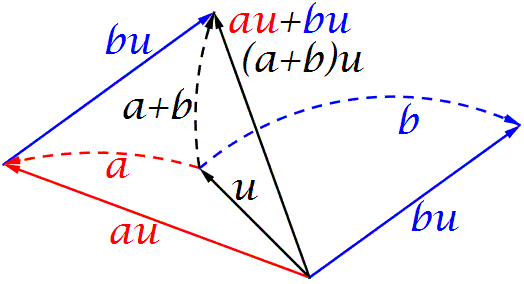
\includegraphics[width=0.5\textwidth]{imagenes/imagenes01/T01IM01.png}
		%\caption{Los dos problemas clásicos del cálculo: trazado de tangentes y áreas bajo curvas.}
	%\end{figure}
		
%varios párrafos encuadrados - explicaciones ad hoc
%\centering{
%\fbox{
%\parbox{0.95\textwidth}{
%varios
%
%$parrafos
%
%dentro
%}
%}
%}
% \justify


%\rotatebox{180}{\leftline{\textcolor{gris}{tararí}}}.